\documentclass[12pt,a4paper]{article}
\usepackage[utf8]{inputenc}
\usepackage{amsmath,amssymb}
\usepackage{booktabs}
\usepackage{array}
\usepackage{graphicx}
\usepackage{hyperref}
\usepackage{geometry}
\usepackage{xcolor}
\geometry{margin=1in}
\setlength{\parskip}{0.8em}
\setlength{\parindent}{0pt}

\title{Guidebook to Exercise 3: \textit{Computational Graphs}}
\author{Prof. Dr. Ivan Habernal \\ Yassine Thlija}
\date{2025-10-30}

\begin{document}

\maketitle

\section{Introduction}
A \emph{computational graph} is a directed acyclic graph (DAG) where nodes represent elementary operations or values (constants, parameters) and edges represent the flow of scalar (or vector) values between operations. Computational graphs are the foundation of automatic differentiation and backpropagation in neural networks.

Example from Lecture 3:

\begin{center}
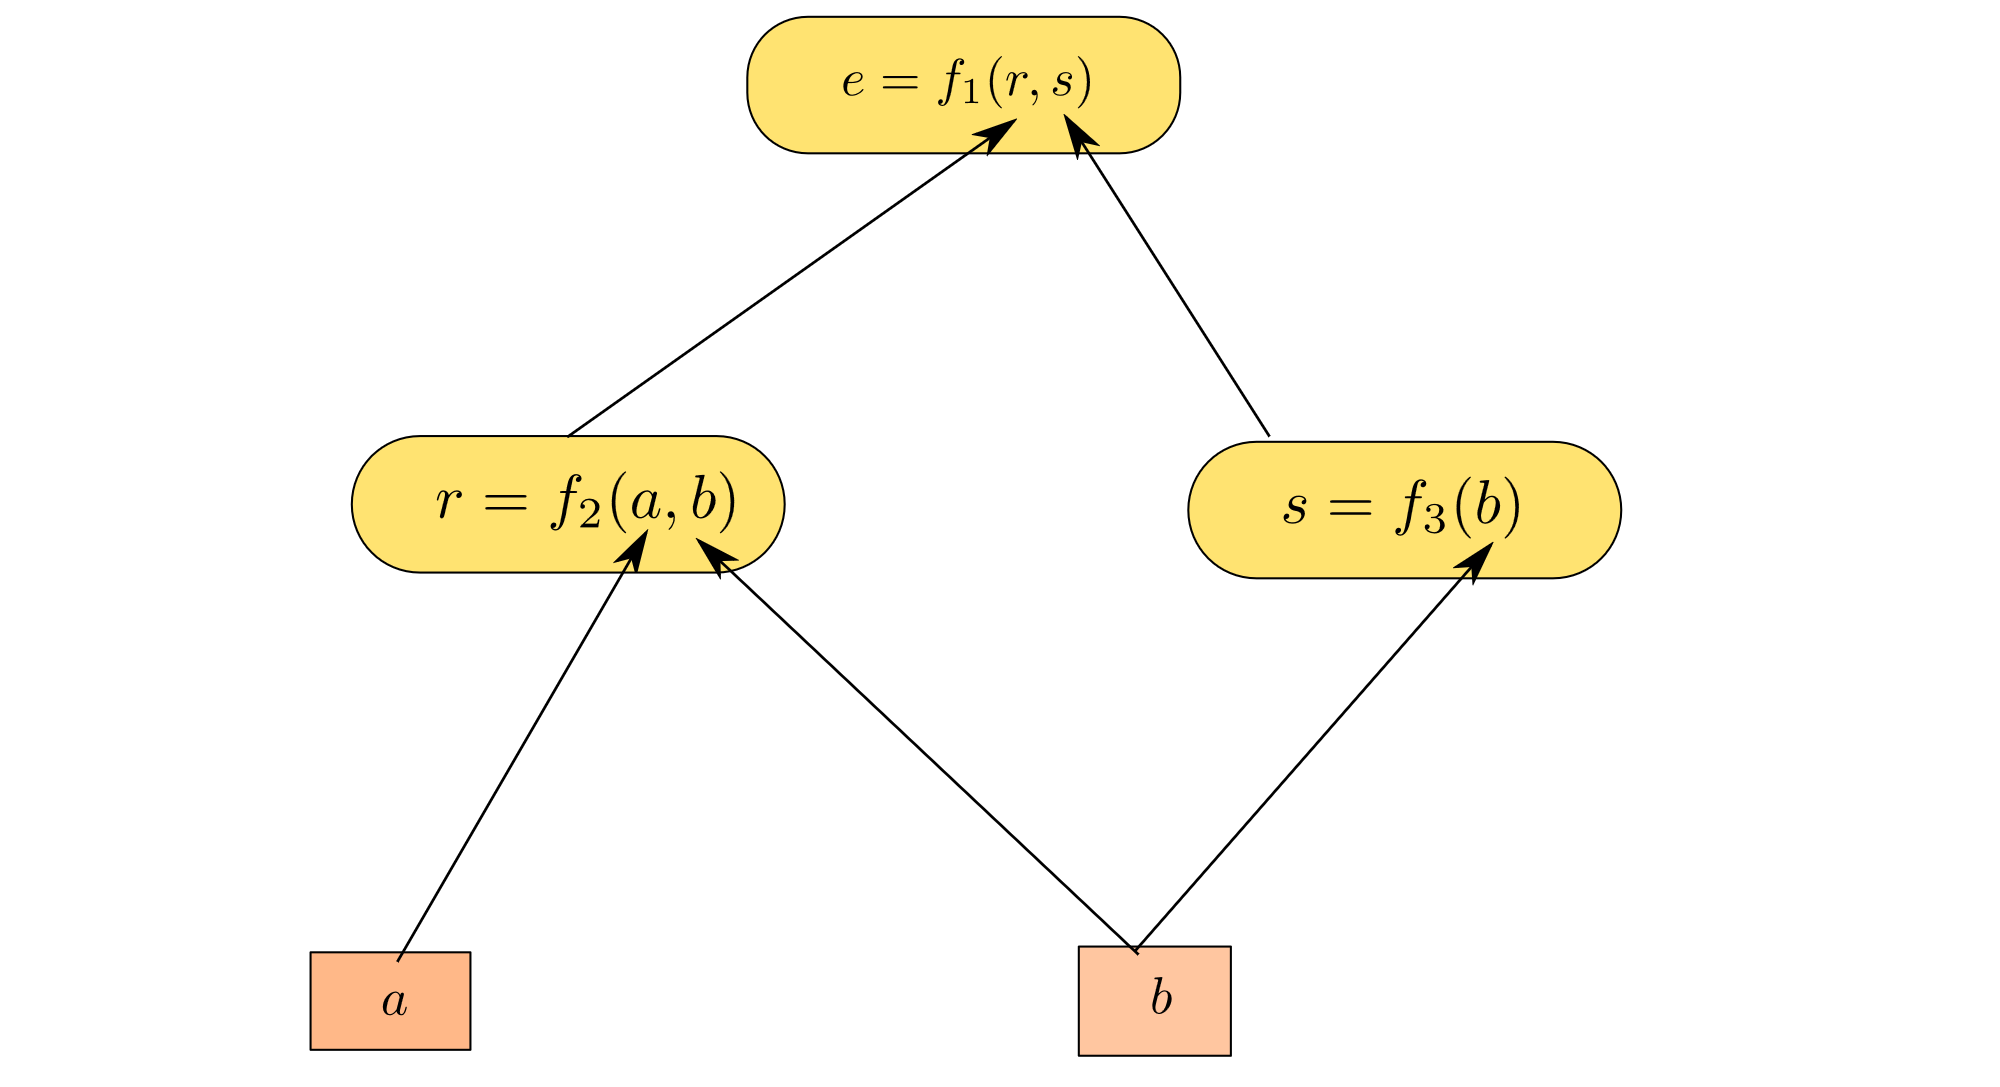
\includegraphics[scale=0.2]{compu_graph_lect3_mod.png}
\end{center}

\section{Some definitions}
\subsection{Nodes and values}
We will work with scalar computational graphs. A \emph{node} $n$ computes a scalar value $v_n$. There are two elementary node types:
\begin{itemize}
    \item \textbf{Leaf node (constant node)}: represents a numeric constant or input variable, e.g. $a$, $b$, $x$. Its value is fixed for a particular forward pass.
    \item \textbf{Operation node}: computes a function of its argument nodes. Examples include sums, products, differences and compositions (In the exercise we will only be using Sum and Product Nodes).
\end{itemize}

Edges are directed from argument nodes toward the operation node. The root node is the final scalar we are interested in.

\subsection{Forward evaluation}
Given values for leaf nodes, we compute values for internal nodes by evaluating their defining expressions in topological order. 

\textbf{Example:}  
Let $s = a + b$, with $a=1$, $b=2$. Then the forward evaluation gives $s=3$.  

\section{Local partial derivatives}
For an operation node $p$ that takes arguments $x_1,\dots,x_k$ and computes $p=f(x_1,\dots,x_k)$, we define the \emph{local partial derivatives}
\[
\frac{\partial p}{\partial x_i} = \frac{\partial f(x_1,\dots,x_k)}{\partial x_i}.
\]
These are \emph{local} because they describe how $p$ changes when only a single argument $x_i$ changes, with the other arguments held fixed.

\subsection*{Examples}
\begin{enumerate}
    \item \textbf{Sum node:} $s = x_1 + \dots + x_k$ gives 
    \[
    \frac{\partial s}{\partial x_i} = 1 \quad \forall i.
    \]
    \item \textbf{Product node:} $p = \prod_{i=1}^k x_i$ gives
    \[
    \frac{\partial p}{\partial x_i} = \prod_{j\neq i} x_j.
    \]
\end{enumerate}

\textbf{Example:} For $p = a \cdot b \cdot c$, we have:
\[
\frac{\partial p}{\partial a} = b \cdot c, \quad 
\frac{\partial p}{\partial b} = a \cdot c, \quad 
\frac{\partial p}{\partial c} = a \cdot b.
\]

\section{Global derivatives and the generalized chain rule}
Suppose the final scalar of interest (the root) is $y$ and a node in the graph is $u$ with value $v_u$. We want the derivative of $y$ with respect to the value at $u$, denoted
\[
\frac{d y}{d u}.
\]
Because the graph is a DAG, $y$ may depend on $u$ through many distinct paths. The \textbf{generalized chain rule} (also used in backpropagation) states that the global derivative of $y$ with respect to $u$ is the sum over all immediate parents $p$ of $u$ of:
\[
\frac{d y}{d u} = \sum_{p \in \operatorname{Parents}(u)} \frac{\partial p}{\partial u}\cdot \frac{d y}{d p}.
\]
If $u$ is the root node, then $\frac{dy}{du}=1$.

\section{Some Examples}

\subsection{Example 1: A Simple Graph}
Let
\[
a=2, \quad b=3, \quad c = a+b, \quad y = c^2.
\]

\textbf{Forward pass:}
\[
c = 5, \quad y = 25.
\]

\textbf{Backward pass (chain rule demonstration):}
\[
\frac{dy}{dc} = 2c = 10, \quad
\frac{dc}{da} = 1, \quad \frac{dc}{db} = 1.
\]
Thus:
\[
\frac{dy}{da} = \frac{dy}{dc} \cdot \frac{dc}{da} = 10, \quad
\frac{dy}{db} = \frac{dy}{dc} \cdot \frac{dc}{db} = 10.
\]
\clearpage
\subsection{Example 2: Multiplicative Graph}
Let
\[
x=1, \quad y=2, \quad z = x \cdot y, \quad r = z + y.
\]

\textbf{Forward:}
\[
z = 2, \quad r = 4.
\]

\textbf{Backward:}
\[
\frac{dr}{dz}=1, \quad \frac{dr}{dy}=1.
\]
Also,
\[
\frac{dz}{dx}=y=2, \quad \frac{dz}{dy}=x=1.
\]
Then:
\[
\frac{dr}{dx} = \frac{dr}{dz}\frac{dz}{dx} = 2, \quad
\frac{dr}{dy} = \frac{dr}{dz}\frac{dz}{dy} + 1 = 1 + 1 = 2.
\]

\section{If you want to dive deeper}
Try building computational graphs for the following:
\begin{itemize}
    \item $y = (a+b)(b+c)$
    \item $y = (x_1 + x_2 + x_3)^2$
    \item $y = x \cdot (x + 2)$
\end{itemize}
For each, perform both forward and backward passes and verify your gradients symbolically.


\end{document}
